\chapter{Experimental characterization of the DOE/SNL Reference Model 2
    cross-flow turbine} \label{chap:RM2}

In the study described in this chapter, a DOE/SNL Reference Model 2 cross-flow
MHK turbine was designed and built to 1:6 scale, then its performance, Reynolds
number dependence, and near-wake characteristics were measured using the turbine
test bed. Note most of the content here has been taken from
\cite{Bachant2016-RM2-paper}.

The Reference Model Project (RMP), sponsored by the US Department of Energy
(DOE), produced six marine hydrokinetic (MHK) technology point designs as
reference models (RMs) to serve as non-proprietary test articles for open
research development, and to benchmark performance and costs for technology
developers \cite{Neary2014, Neary2014a}. Open-source RMP products, along with
supporting documentation, are available at the RMP website
\url{http://energy.sandia.gov/rmp} to facilitate their use in future R\&D
studies by industry, academia, and national laboratories. These products
include: Technical specifications and computer-aided design (CAD) files for each
RM device to allow exact replication for physical and numerical modeling
studies; resource site information used to design each RM device; and references
to physical modeling data sets that can be used to validate numerical modeling
design and analysis tools.

\nomenclature{DOE}{US Department of Energy.}

Reference Model 2 (RM2) is a dual-rotor, vertical-axis cross-flow hydrokinetic
(river) turbine that was designed to operate in a reach of the lower Mississippi
River near Baton Rouge, Louisiana \cite{Barone2011, Neary2011}. The rotor has
three tapered blades and a relatively low solidity $Nc/(\pi D)$ or
chord-to-radius ratio $c/R \approx 0.1$. A preliminary analysis with Sandia's
CACTUS vortex line numerical model \cite{Murray2011} predicted an individual
rotor's full-scale performance coefficient to be $C_P=0.47$ at 1 m/s flow speed
and a tip speed ratio $\lambda \equiv \frac{\omega R}{U_\infty} = 3.15$
\cite{Barone2011}, where $\omega$ and $R$ are the rotor's angular velocity and
radius, respectively. Note that the RM2 rotor solidity would be considered
moderate to high for a wind turbine, whose $c/R$ values typically range from
0.05 to 0.09, but MHK rotors are typically higher solidity since they must
withstand approximately an order of magnitude higher torque in typical flows,
necessitating relatively larger blades to meet strength and fatigue life
requirements.

An initial experimental measurement campaign with a 1:15 scale RM2 rotor
conducted at the Saint Anthony Falls Laboratory (SAFL) at the University of
Minnesota resulted in maximum power coefficient of approximately 5\% at $\lambda
= 2.2$ \cite{Hill2014}. This discrepancy between numerical and physical model
performance prompted the experimental measurements presented here, namely due to
the low Reynolds number---$Re_D = U_\infty D / \nu$, where $U_\infty$ is the
free stream velocity, $D$ is the rotor diameter, and $\nu$ is the fluid
kinematic viscosity---of the 1:15 scale tests, which were performed at $Re_D
\sim 10^5$.

The effect of Reynolds number on average power output was shown to be
significant on the 2 m Sandia Research Darrieus turbine in wind tunnel testing
\cite{Blackwell1976}: The maximum power coefficient, $C_{P_{\max}}$, increased
with Reynolds number, $Re_c=\lambda U_\infty c / \nu$ (based on blade chord
rather than diameter, though these are approximately proportional since optimal
tip speed ratio correlates inversely with solitidy and therefore chord length),
along with a shift of the location of $C_{P_{\max}}$ toward lower tip speed
ratios due to delayed blade stall. The effects of Reynolds number were quite
dramatic over a relatively small range of $Re_c \approx 1.1 \times 10^5$--$2.9
\times 10^5$. More recently, Bachant and Wosnik \cite{Bachant2014,
Bachant2016-RVAT-Re-dep} showed that performance and near-wake characteristics
of a high solidity cross-flow turbine become Reynolds number independent at
$Re_D \approx 10^6$ or $Re_c \approx 2 \times 10^5$.

As part of the engineering process it is generally less expensive to assess
designs via numerical rather than physical models. However, it is
important---especially when dealing with fluid dynamics where the ``exact''
physics cannot be resolved with even the most advanced computers---that
numerical models be validated against experimental data. It is uncertain whether
numerical models validated with physical model data obtained at low Reynolds
numbers should be considered validated at all, since the scale at which the
model will be applied for real world design problems is orders of magnitude
larger. One way to overcome this uncertainty is to show that the scaled physical
model test has become Reynolds number independent, so validation efforts are
relevant at full-scale, which was the strategy employed here.

The main objective of the present study was to acquire a new experimental
dataset for the RM2 turbine at sufficiently high Reynolds numbers to be relevant
to full-scale physical and numerical modeling. It was hypothesized that the
parasitic losses from rotor blade support struts could play an important role in
overall turbine performance, especially for a lower solidity turbine that
operates at higher tip speed ratios. Thus, the parasitic torque from strut drag
was measured without blades, then deliberately and significantly increased in
the physical model to provide data to investigate its importance. The velocity
field in the near-wake of the turbine was then measured to compare with
measurements from a higher solidity rotor in the same experimental setup
\cite{Bachant2015-JoT}, and to provide validation data for numerical models that
predict wake flows, which determine turbine--turbine interaction and optimal
spacing for turbine arrays. This dataset, along with the code for processing and
visualization, has been made publicly available (licensed via Creative Commons
CC-BY for data and MIT license for code) as a Git repository on GitHub
(\url{https://github.com/UNH-CORE/RM2-tow-tank}) and as a citable archive with a
digital object identifier (DOI) \cite{Bachant2016-RM2-data}.


\section{Survey of validation data and usage}

To provide perspective on where this investigation fits amongst past studies,
including those in previous chapters, a selection of measured performance data
in the literature and its usage in numerical model validation is presented in
Table~\ref{tab:validation-data}. Turbine diameter Reynolds numbers spanned from
small laboratory scale ($Re_D \sim 10^5$) all the way to full scale ($Re_D \sim
10^7$). Individual blade forces were only measured in two of the
experiments---Strickland et al. \cite{Strickland1981} and Laneville and Vitecoq
\cite{Laneville1986}. There has been nearly equal attention given to the
eggbeater-shaped Darrieus rotor and the straight-bladed H-rotor. The performance
of a large scale H-rotor with tapered blades, the VAWT 850 \cite{Mays1990}, has
also been measured.

\begin{table}
    \centering

    \begin{tabular}{c|c|c|c|c|c}
        Name & Rotor type & $N_\mathrm{b}$ & $c/R$ & $Re_D$ & Used in \\
        \hline
        Sandia 2 m \cite{Blackwell1976} &  Darrieus  & 2--3 & 0.06--0.09 & $\sim 10^6$ & \cite{Roh2013,Bedon2014} \\
        Sandia 5 m \cite{Sheldahl1977} &  Darrieus  & 3 & 0.08 & $\sim 10^6$ & \cite{Antheaume2008,Bedon2014} \\
        Sandia 17 m \cite{Worstell1978} & Darrieus  & 2 & 0.06 & $\sim 10^7$ & \cite{Para1988,Orlandi2015,Bedon2014} \\
        Sandia 34 m \cite{Ashwill1992} & Darrieus  & 2 & 0.05 & $\sim 10^7$ & \cite{Liu1992,Murray2011,Bedon2014}  \\
        Strickland et al. \cite{Strickland1981} & H & 1--3 & 0.15 & $\sim 10^5$ & \cite{Ponta2001,Scheurich2011b} \\
        Laneville and Vitecoq \cite{Laneville1986} & H & 2 & 0.13 & $\sim 10^6$ & \cite{Amet2009} \\
        Howell et al. \cite{Howell2010} & H & 2--3 & 0.33 & $\sim 10^5$ & \cite{Joo2015} \\
        Mertens \cite{Mertens2003} & H & 2 & 0.21 & $\sim 10^5$ & \cite{Orlandi2015} \\
        VAWT 850 \cite{Mays1990} & Tapered H & 2 & 0.05 & $\sim 10^7$ & \cite{Murray2011} \\
        UNH-RVAT \cite{Bachant2014-RVAT-baseline} & H & 3 & 0.28 & $\sim 10^6$ & \cite{Michelen2014} \\
        RM2 (present) & Tapered H & 3 & 0.07--0.12 & $\sim 10^6$ &
    \end{tabular}

    \caption{Selected measured performance data and its usage for numerical
        model validation. Note that individual blade forces were measured in the
        Strickland et al. and Laneville and Vitecoq experiments.}

    \label{tab:validation-data}
\end{table}

In general, there have been more experiments done with low $c/R$ rotors. These
rotors are easier to model, since unsteady dynamic effects are less influential
on the overall performance \cite{Strickland1981}. This is apparent when
examining the effectiveness of numerical models that rely on static foil
coefficient input data, e.g., streamtube and vortex models, which are most
applicable for $c/R \leq 0.1$. For example, Bedon et al.~\cite{Bedon2014}
used a double multiple streamtube momentum model without dynamic stall
corrections to evaluate the effectiveness of various foil coefficient databases
against the Sandia Darrieus turbine experimental data. Despite using such a
simple model, performance predictions were quite accurate in most conditions
except at low tip speed ratio for the 2 m turbine, which had the highest $c/R$
of all the Sandia rotors, making the dynamic effects more important. This
highlights the need for more validation data for higher solidity rotors to
ensure numerical models are robust enough to explore unique cross-flow turbine
designs, especially as the MHK concepts mature.

The UNH-RVAT, for which the performance, near-wake, and Reynolds number
dependence of was investigated using the same experimental setup as the study
here \cite{Bachant2015-JoT, Bachant2016-Energies}, was an H-rotor of 1 m height
and 1 m diameter. The UNH-RVAT experimental datasets are also openly available
\cite{Bachant2014-RVAT-baseline, Bachant2016-RVAT-Re-dep}, and provide an
interesting comparison for the near-wake dynamics of a rotor similar in size to
the 1:6 scale RM2, but with non-tapered blades and a high solidity $c/R = 0.28$.


\section{Test bed external regeneration resistor modification}

During the UNH-RVAT Reynolds number dependence experiment described in
Chapter~\ref{chap:Re-dep}, it was noted that the turbine test bed's Kollmorgen
AKD servo drive was nearly reaching its 200 W internal power dissipation limit
for the higher speed tows. Since the RM2 was expected to produce more power,
before this experiment an Kollmorgen BAR1000-15 external regeneration resistor
was added to the system to bring the power dissipation capacity up to 1 kW,
ensuring this would not be a limiting factor for testing the RM2 at higher tow
speeds.


\section{Turbine model details}

Geometric parameters for the 1:6 scale RM2 rotor were taken from the RM2 design
report \cite{Barone2011}, with the exception of the shaft diameter, which was
scaled from the SAFL RM2 model \cite{Hill2014}. Values for both the 1:6 and
full-scale designs are presented in Table~\ref{tab:rm2-geom} and a drawing and
photo of the turbine is shown in Figure~\ref{fig:rm2}. The rotor
components---blades, struts, shaft, and center hub sections---were fabricated
from 6061-T6 aluminum, which was hardcoat anodized per MIL-8625-A, type III,
class 2 specifications. CAD models and manufacturing drawings for the turbine
are available from \cite{Bachant2015-RM2-CAD}. Note that after fabrication the
turbine parts were inspected both by the manufacturer and in-house to ensure
parts were within the design tolerances, the results from which are available in
the experimental repository \cite{Bachant2016-RM2-data}.

\begin{table}
    \centering
    \begin{tabular}{l|l|l}
        & Full-scale & Model (1:6) \\
        \hline
        Diameter (m)   & 6.450 & 1.075 \\
        Height (m)     & 4.840 & 0.8067 \\
        Blade root chord (m) & 0.4000 & 0.06667 \\
        Blade tip chord (m)  & 0.2400 & 0.04000 \\
        Blade profile & NACA 0021 & NACA 0021 \\
        Blade mount & 1/2 chord & 1/2 chord \\
        Blade pitch (deg.) & 0.0 & 0.0 \\
        Strut profile & NACA 0021 & NACA 0021 \\
        Strut chord (m) & 0.3600 & 0.06000 \\
        Shaft diameter (m) & 0.2540 \cite{Beam2011} or 0.4160 \cite{Hill2014} & 0.06350\\
    \end{tabular}
    \caption{RM2 turbine geometric parameters for full and 1:6 scale models.}
    \label{tab:rm2-geom}
\end{table}

The rotor was 1.075 m in diameter and 0.8067 m tall, with blade chords that
taper from 0.067 m at the roots, or half-span, to 0.04 m at the tips, varying
the chord-to-radius ratio $c/R$ from 0.12 to 0.07 (0.1 average). The rotor was
therefore approximately at the threshold between high and low solidity
\cite{Strickland1981,Fiedler2009}, which presents a unique validation case not
yet seen in the literature. The RM2 is conceptually similar to the VAWT 850
\cite{Mays1990} which also had tapered blades, but the RM2 has a moderately high
$c/R$ to more accurately represent typical MHK rotors, which presents a
challenge for numerical modeling.

For investigating the effects of support strut drag losses, a set of cylindrical
covers were designed to slip over the struts, which provided a deliberate and
significant increase in strut drag. Endcaps were also fabricated to allow the
high drag strut cover configuration to be operated without blades. A drawing of
the strut covers is shown in Figure~\ref{fig:covers}.

\begin{figure}
    \centering

    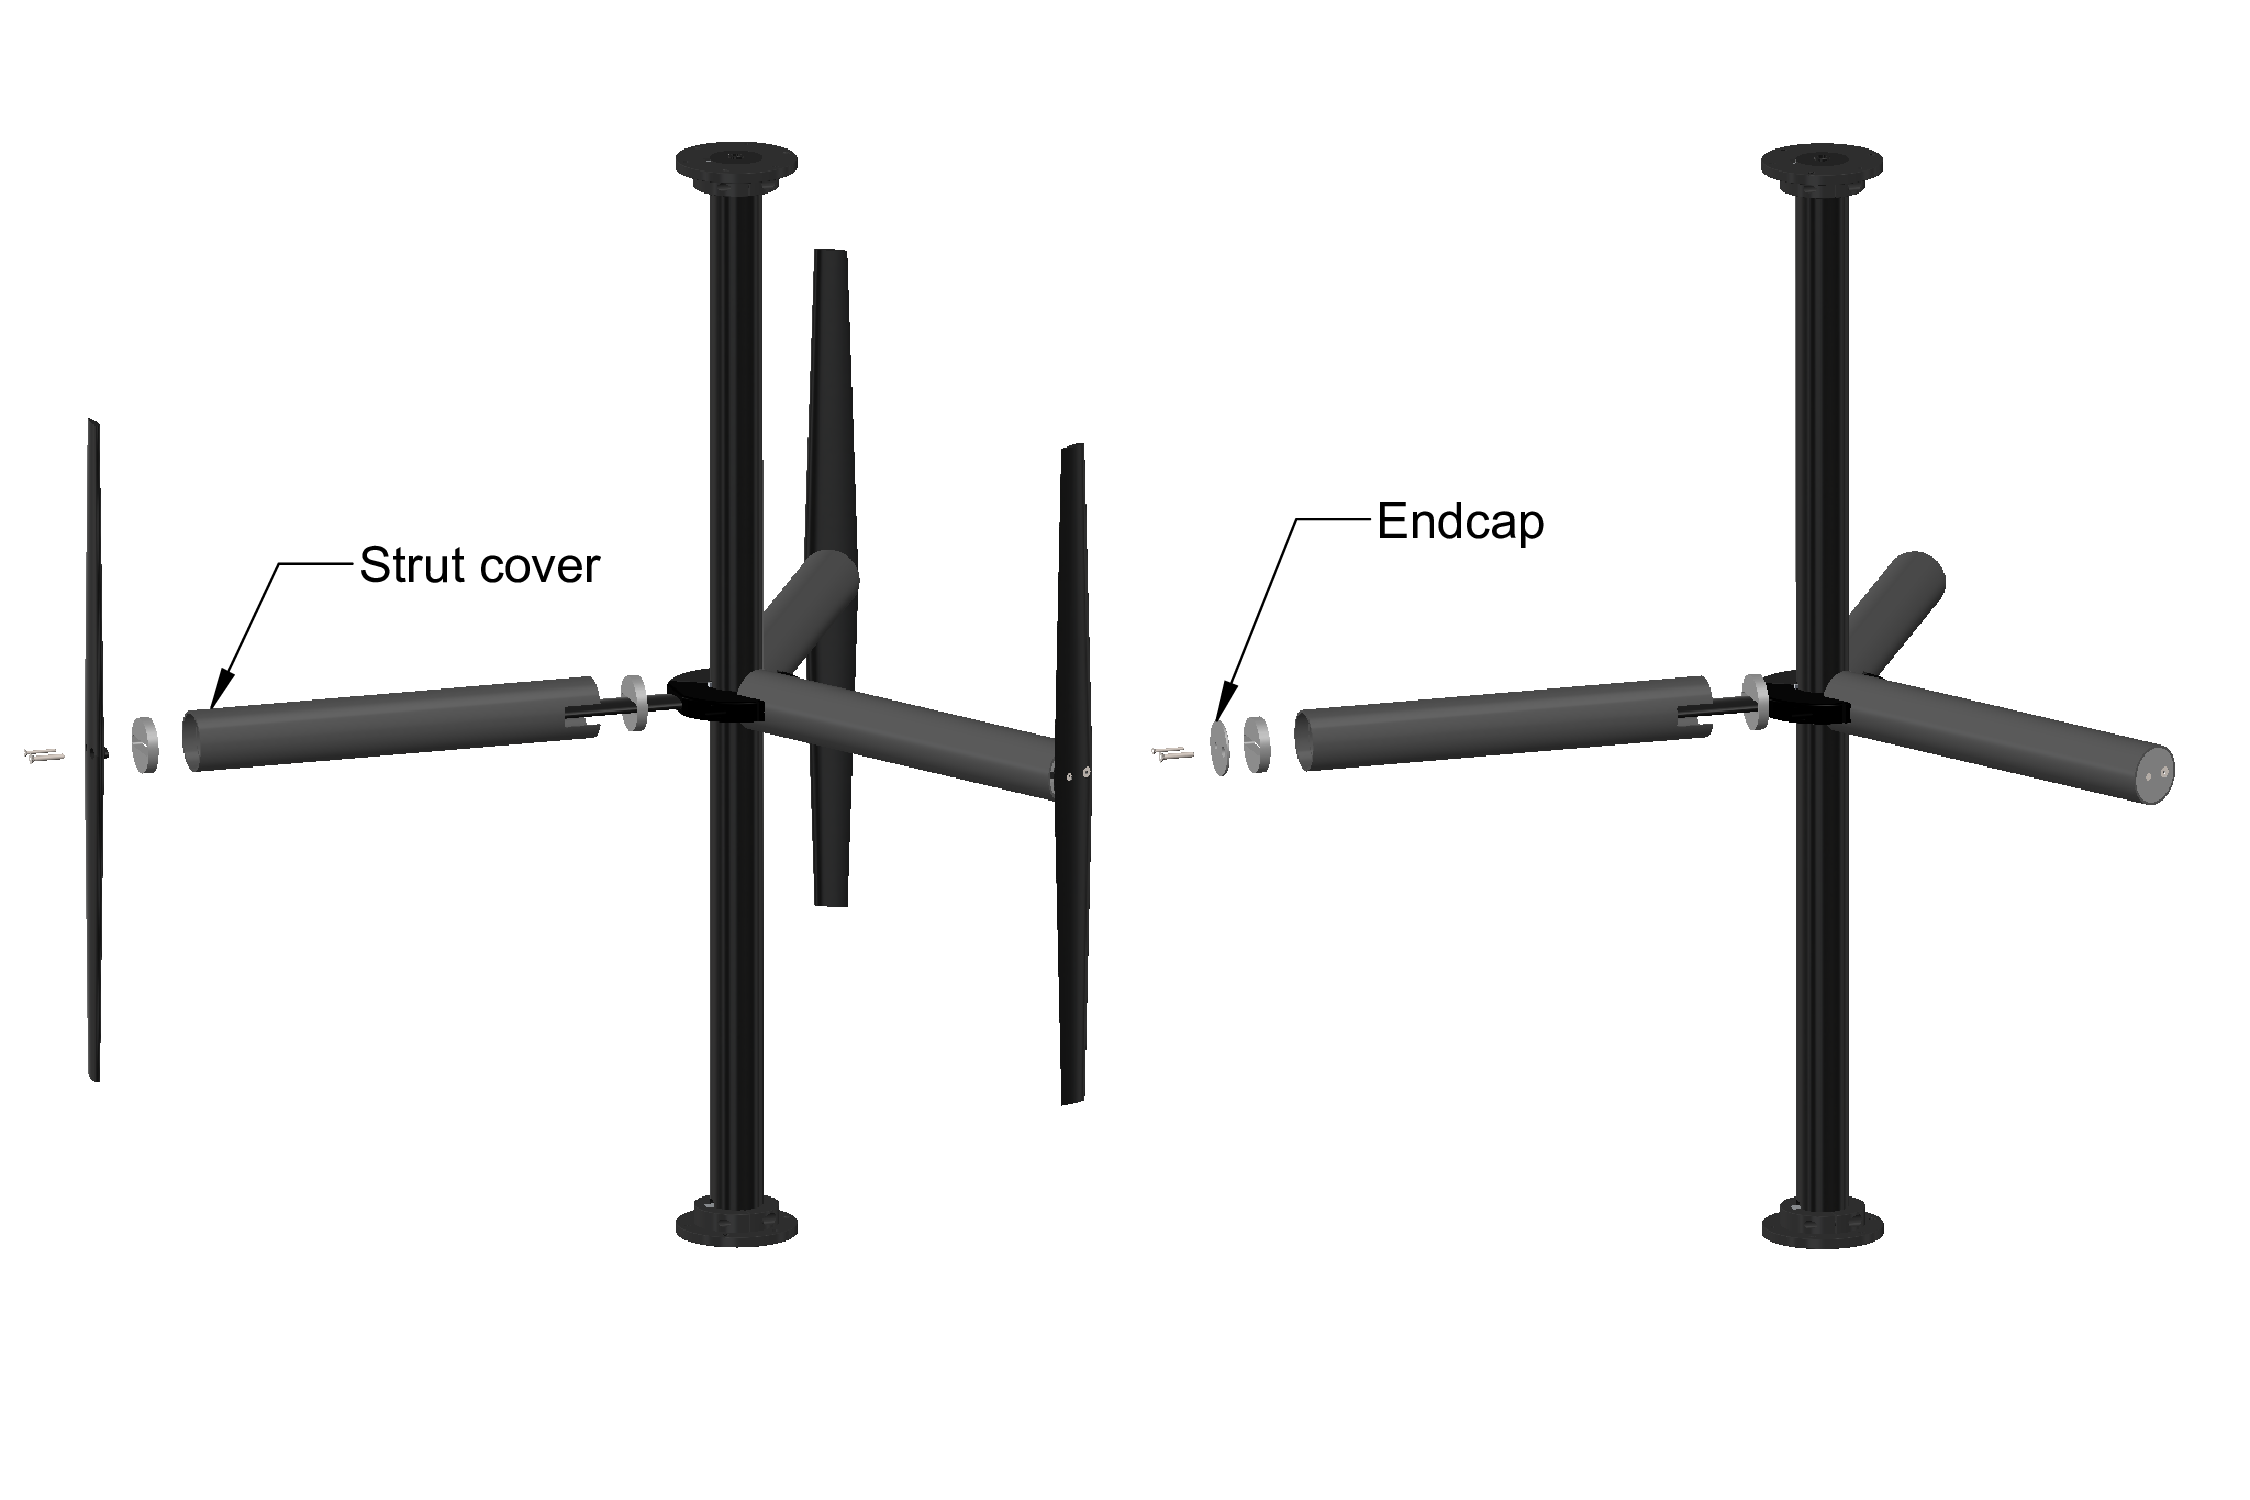
\includegraphics[width=0.95\textwidth]{RM2-strut-covers}

    \caption{A drawing of the high drag strut cover configuration with and
        without blades.}

    \label{fig:covers}
\end{figure}


\section{Test parameters}

Like the experiments described in Chapter~\ref{chap:RVAT-baseline} and
Chapter~\ref{chap:Re-dep}, data collection runs were separated into individual
tows, for which all independent variables---tow speed, tip speed ratio, velocity
probe position---were held constant. These runs were grouped into logical test
matrix ``sections,'' in which typically a single independent variable was
varied. Test matrix section names and descriptions are provided in the
\texttt{README.md} file of the experimental data and code repository
\cite{Bachant2016-RM2-data}. Tow speed and their corresponding turbine diameter
and blade chord Reynolds numbers are presented in Table~\ref{tab:rm2-re}.

\begin{table}
    \centering
    \begin{tabular}{c|c|c|c|c}
        Tow speed (m/s) & $Re_D$ & $Re_{c_\mathrm{tip}}$ & $Re_{c_\mathrm{root}}$ & $Re_{c_\mathrm{mid}}$\\
        \hline
        0.4 & $4.3 \times 10^5$ & $5.0 \times 10^4$ & $8.3 \times 10^4$ & $6.6 \times 10^4$ \\
        0.6 & $6.5 \times 10^5$ & $7.4 \times 10^4$ & $1.2 \times 10^5$ & $9.9 \times 10^4$ \\
        0.8 & $8.6 \times 10^5$ & $9.9 \times 10^4$ & $1.7 \times 10^5$ & $1.3 \times 10^5$ \\
        1.0 & $1.1 \times 10^6$ & $1.2 \times 10^5$ & $2.1 \times 10^5$ & $1.7 \times 10^5$ \\
        1.2 & $1.3 \times 10^6$ & $1.5 \times 10^5$ & $2.5 \times 10^5$ & $2.0 \times 10^5$ \\
    \end{tabular}

    \caption{Turbine diameter and approximate average blade chord Reynolds
        numbers $Re_c \equiv \lambda U_\infty c / \nu$ at blade tip, root, and
        mid-span, corresponding to various tow speeds at $\lambda=3.1$.}

    \label{tab:rm2-re}
\end{table}

Wake measurements were all performed at 1 m downstream, which corresponds to
$x/D = 0.93$. The cross-stream and vertical coordinates are shown in
Figure~\ref{fig:coordinates}. Altogether 750 tows were performed and included in
the experimental database.

\begin{figure}
    \centering

    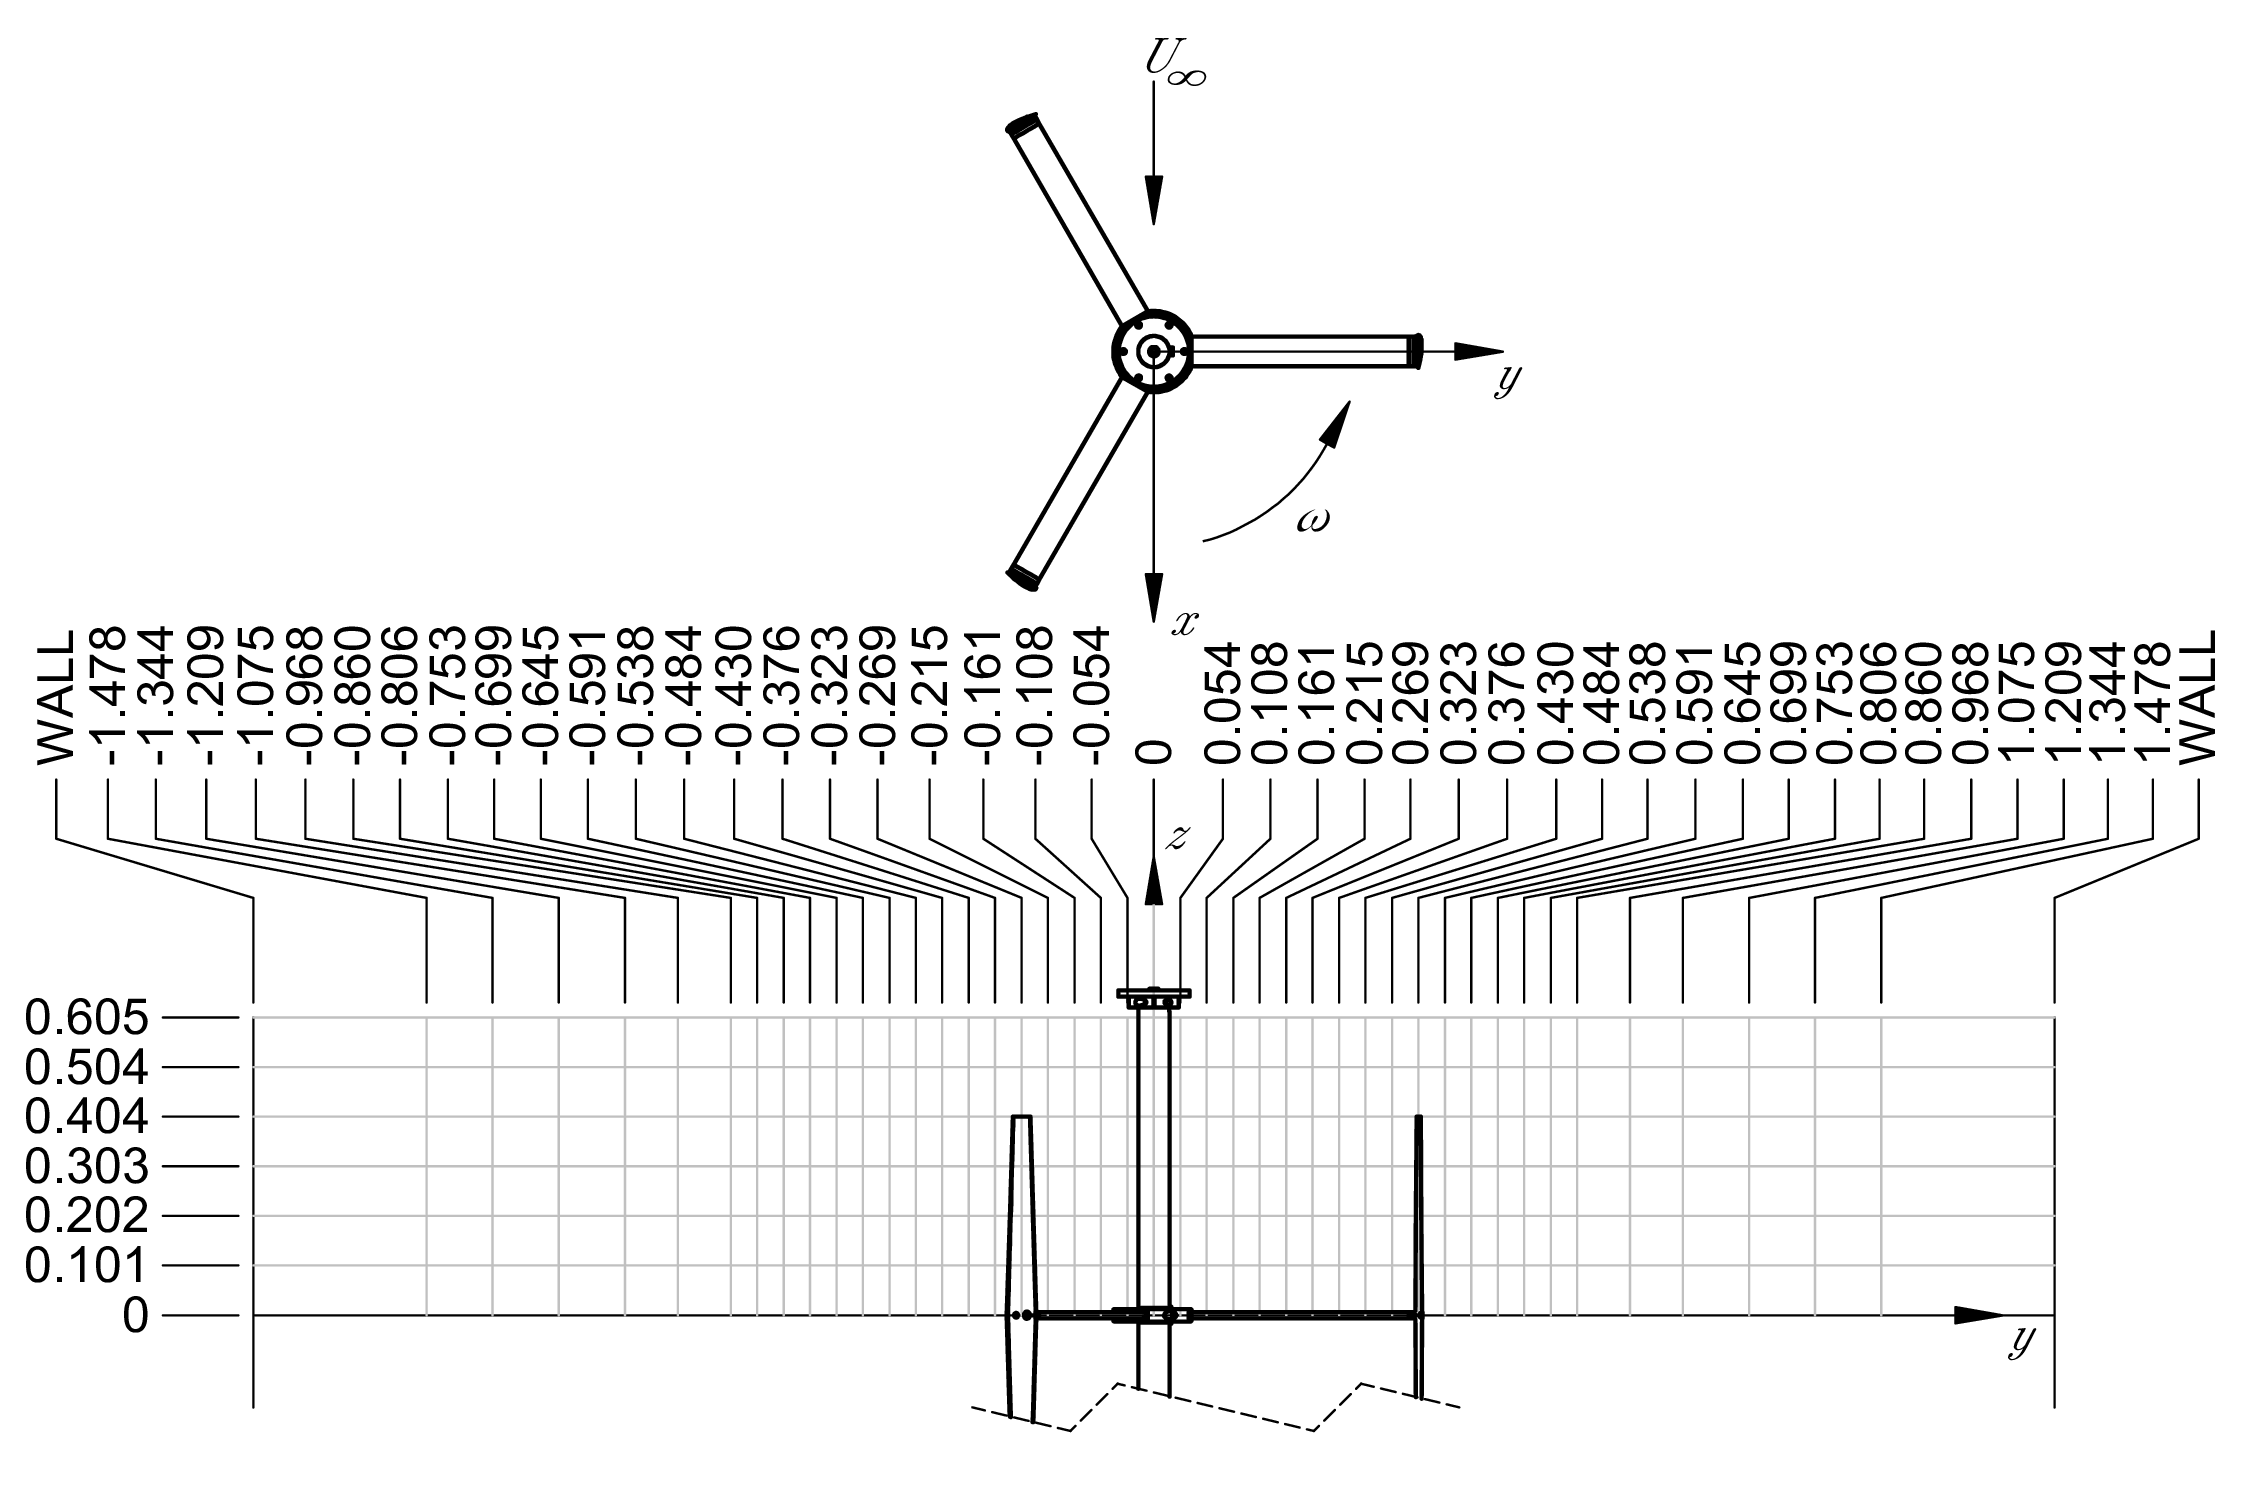
\includegraphics[width=\textwidth]{RM2-coord-sys}

    \caption{RM2 wake measurement coordinate system and cross-stream/vertical
        coordinates. All dimensions are in meters.}

    \label{fig:coordinates}
\end{figure}


\section{Data processing}

For each tow speed, a relevant quasi-steady duration was selected by manually
inspecting a plot of the $C_P$ time series. This interval was then truncated to
include a whole number of blade passages. Relevant statistics were then
calculated over this duration.

To calculate turbine RPM from shaft angle, the encoder signal was differentiated
using a second order central difference scheme, after which an 8 sample wide
moving average smoothing filter was applied to match the noise level present in
the redundant turbine RPM measurement from the motion controller. A similar
approach was used for calculating tow carriage speed $U_\infty$ from carriage
position measurements. Power and drag coefficients were calculated as
instantaneous quantities from the carriage speed as

\begin{equation}
    C_P = \frac{T \omega}{\frac{1}{2} \rho A U_\infty^3}
\end{equation}
and
\begin{equation}
    C_D = \frac{F_\mathrm{drag}}{\frac{1}{2} \rho A U_\infty^2},
\end{equation}
where $\rho$ is the fluid density (assumed to be a nominal 1000
kg/m\textsuperscript{3}) and $A$ is the turbine frontal area $DH$.


\section{Results and discussion}

\subsection{Performance}

Mean rotor power coefficients for multiple Reynolds numbers are plotted versus
tip speed ratio in Figure~\ref{fig:rm2-cp-curves}. In general, $C_P$ increases
with $Re$, along with a reduction in the optimal tip speed ratio, due to the
tendency of foils to stall at higher angles of attack at higher $Re$, and the
higher angle of attack ranges seen by the blades at lower $\lambda$. These
effects diminish with increasing $Re$, which is expected as the blade boundary
layers transition to turbulence closer to the leading edge \cite{Lissaman1983,
McMasters1980, Bachant2016-RVAT-Re-dep}, which helps flow remain attached longer
as it moves against the adverse pressure gradient on the suction side of the
foil. For the experiment reported here, a maximum power coefficient $C_P=0.37$
was reached at $Re_D=1.3 \times 10^6$. Note how at lower tip speed ratios and
Reynolds numbers, $C_P$ becomes significantly negative, which was possible
thanks to the speed control of the experimental setup's servo motor applying
negative torque to the rotor.

\begin{figure}
    \centering

    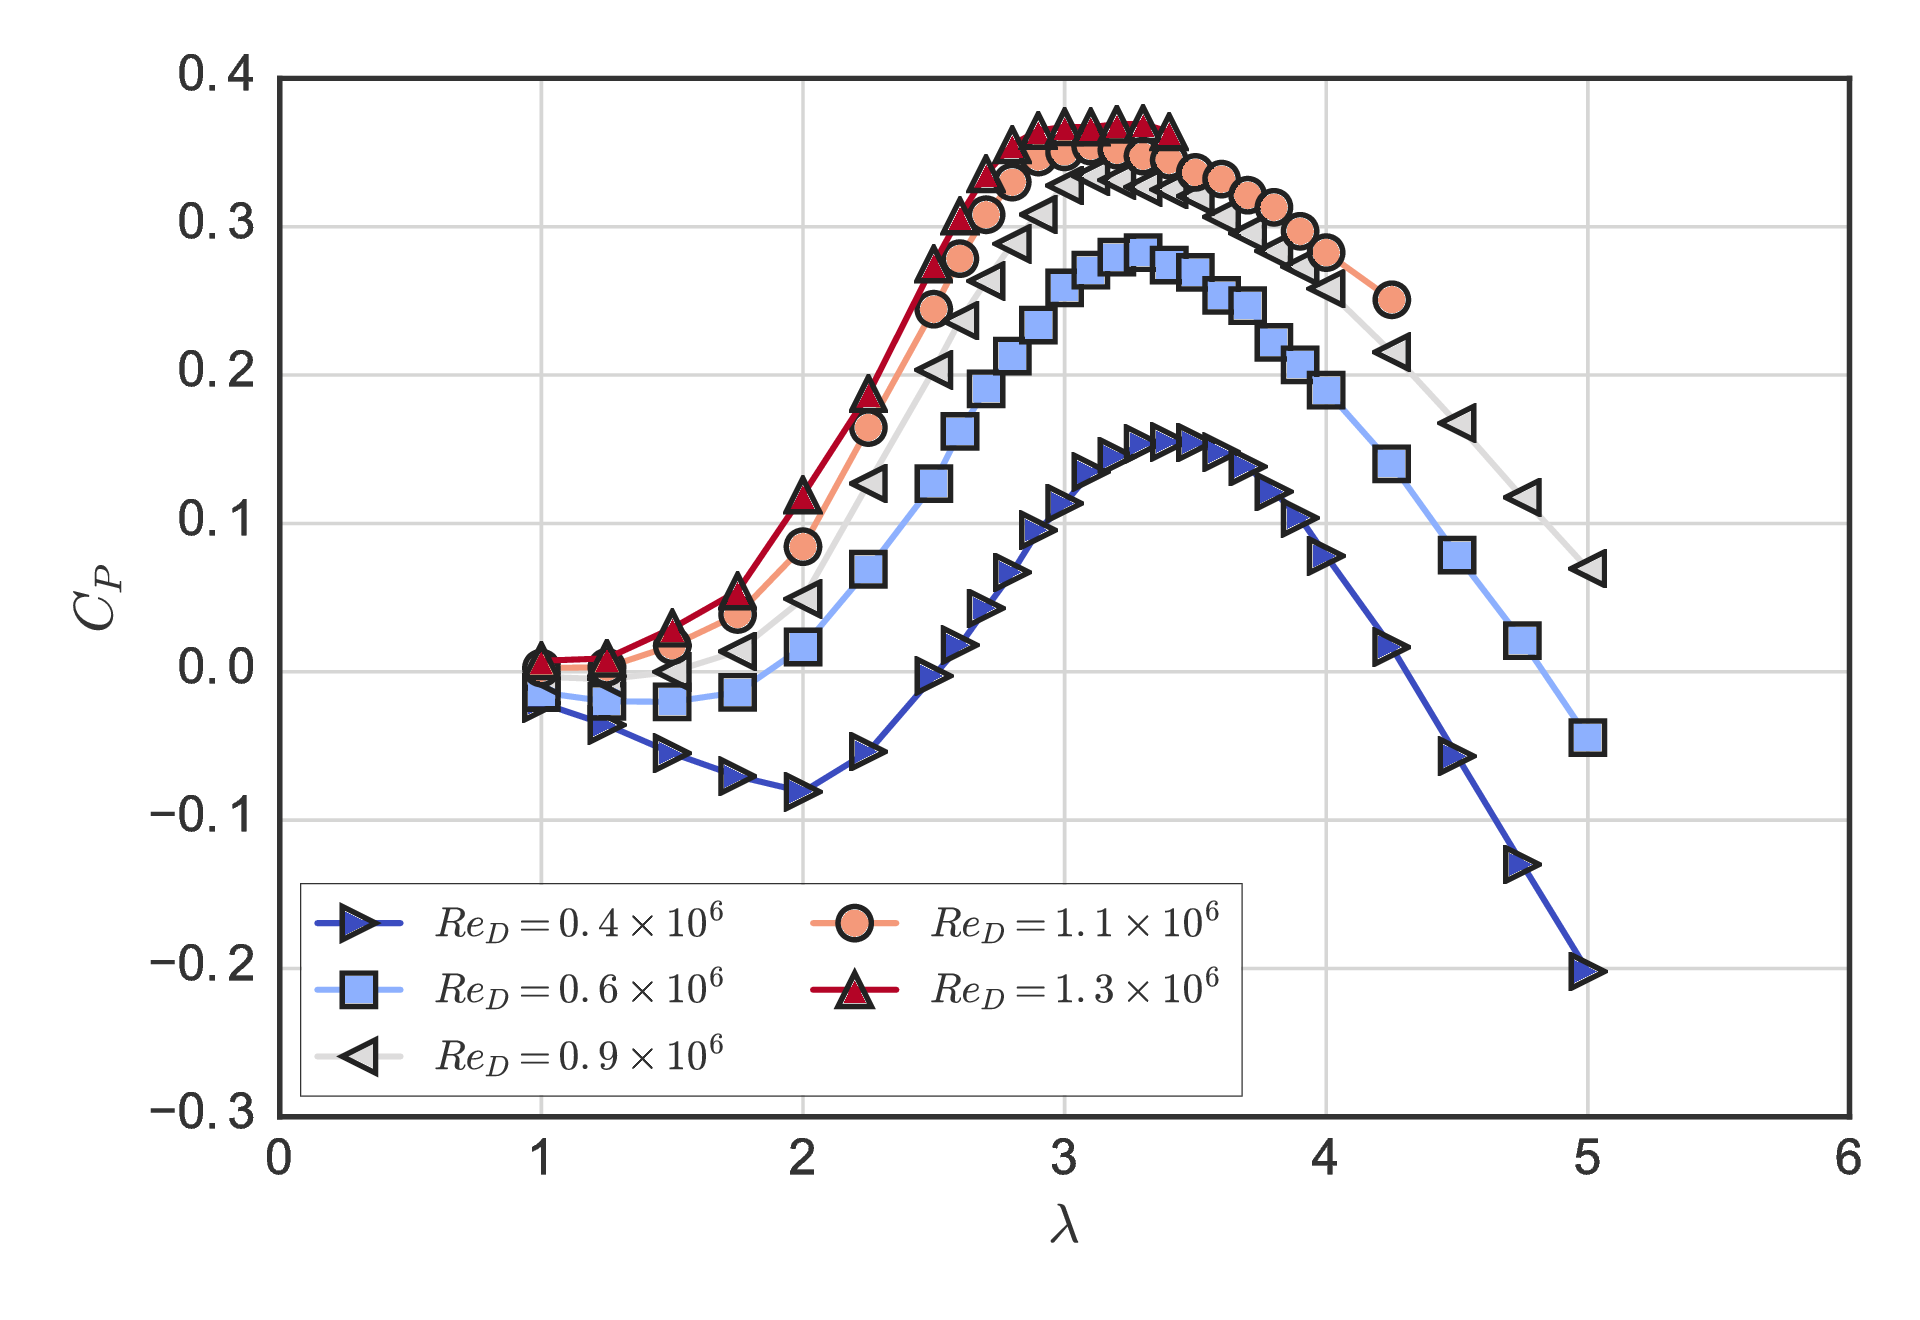
\includegraphics[width=0.75\textwidth]{RM2-tow-tank_cp_curves}

    \caption{Mean rotor power coefficient plotted versus mean tip speed ratio
        for multiple Reynolds numbers.}

    \label{fig:rm2-cp-curves}
\end{figure}

Mean rotor drag coefficients are plotted versus tip speed ratio in
Figure~\ref{fig:rm2-cd-curves}. These $C_D$ curves show little difference
compared to the power coefficient curves, which is most noticeable at low
$\lambda$ and low $Re$. The relative similarity could be attributed to the
effects of stall, where the lift-to-drag ratio on the blades may drop,
decreasing rotor torque, though the total resultant force due to high blade drag
retains a similar component in the streamwise direction. When operating at
maximum power coefficient, $\lambda_0=3.1$, and $Re_D=1.3 \times 10^6$, a rotor
drag coefficient $C_D=0.84$ was measured.

\begin{figure}
    \centering

    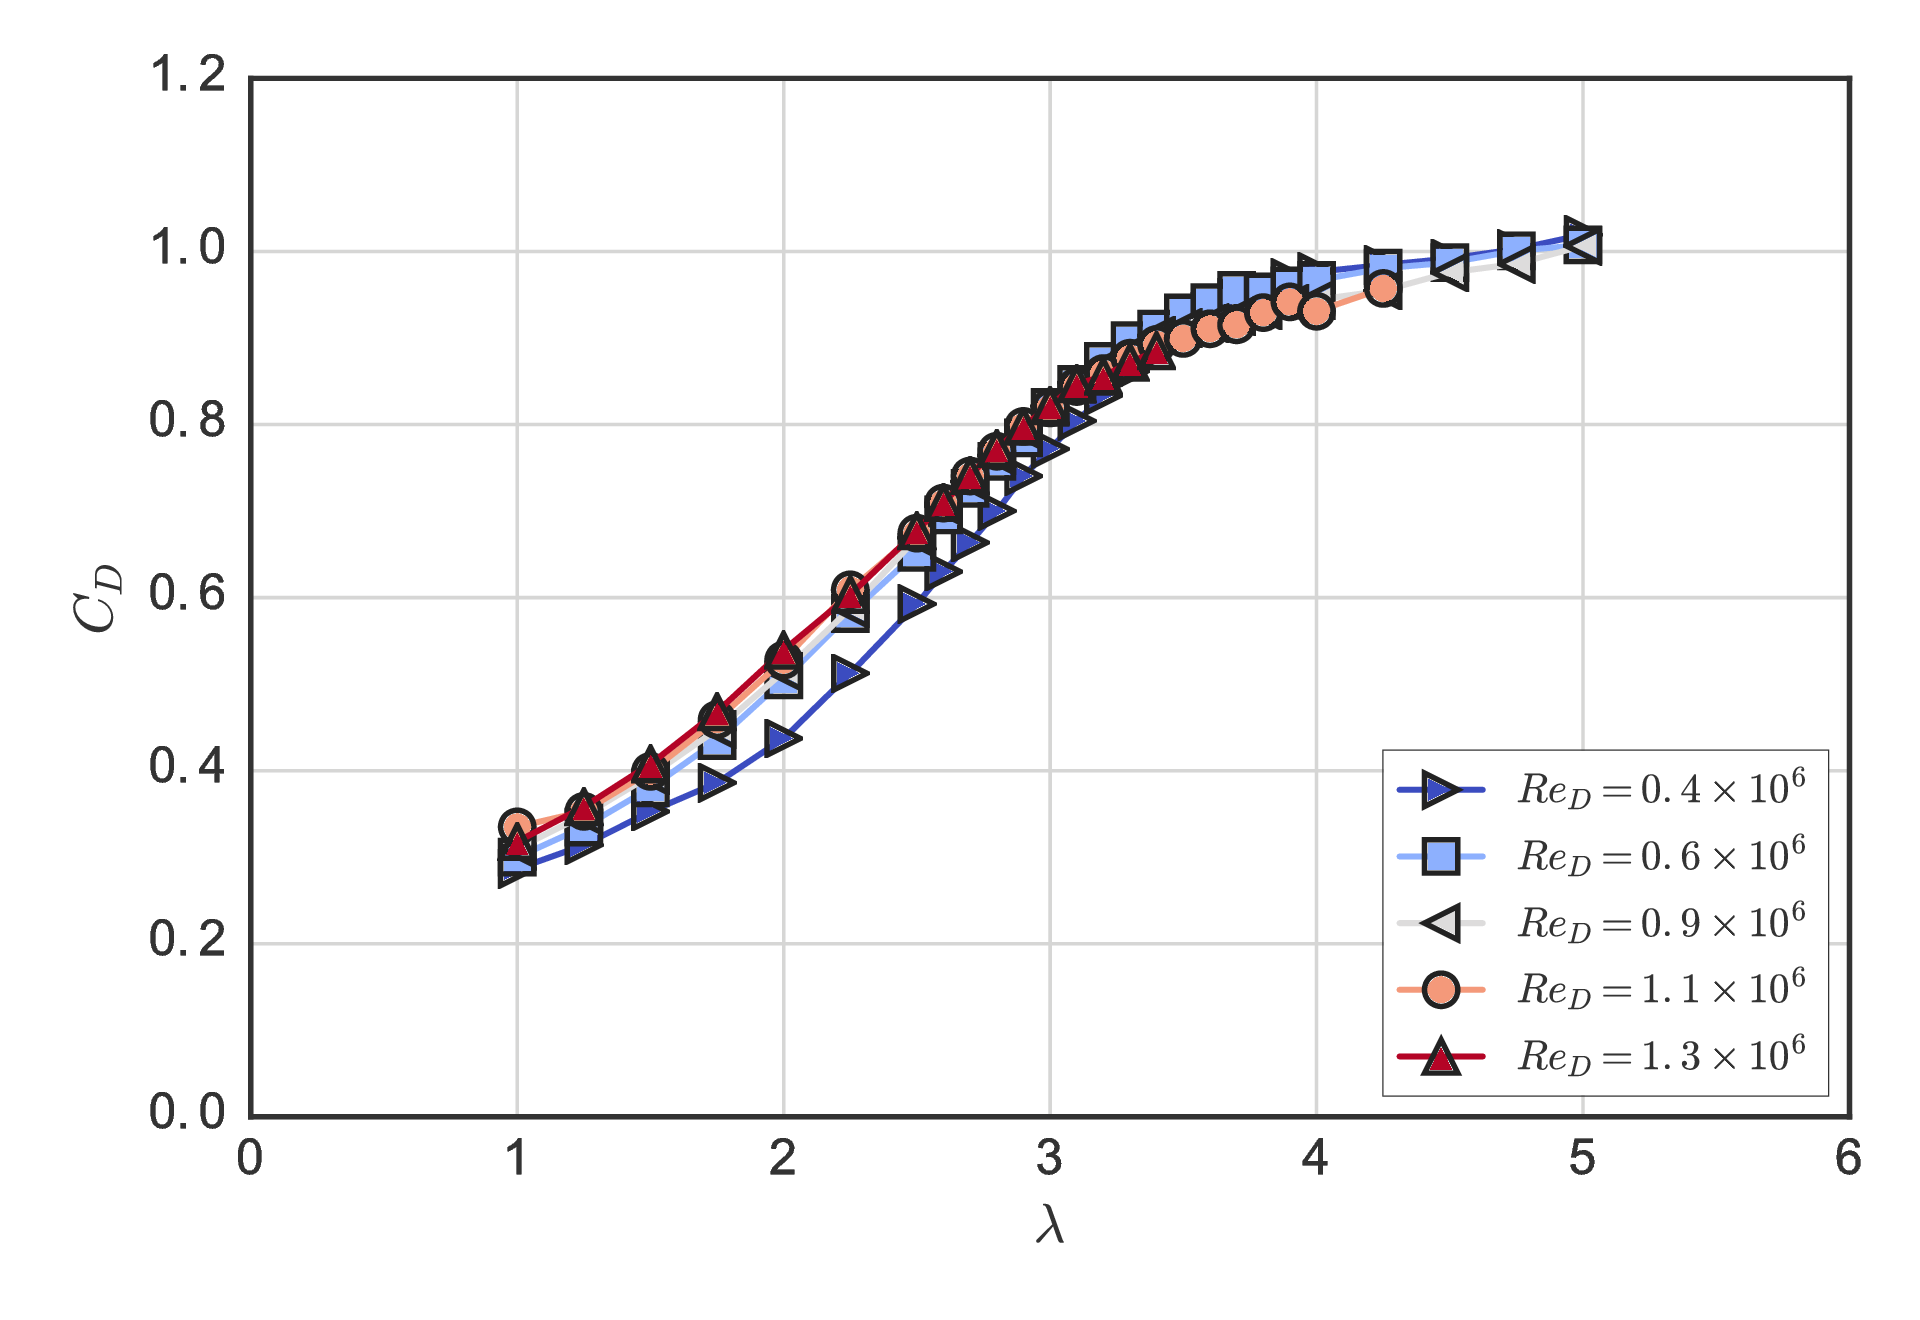
\includegraphics[width=0.75\textwidth]{RM2-tow-tank_cd_curves}

    \caption{Mean rotor drag coefficient plotted versus mean tip speed ratio for
        multiple Reynolds numbers.}

    \label{fig:rm2-cd-curves}
\end{figure}

The power coefficient curves do not collapse exactly onto each other, indicating
Reynolds number dependence, though the differences become relatively small as
$Re$ is increased. Note that the data collection was limited at higher $Re$ and
$\lambda$ due to the unsteady turbine force resonating with the tow carriage
drive belt. However, in contrast to the power coefficient data, the rotor drag
coefficient curves nearly collapse onto each other for $Re_D \ge 0.6 \times
10^6$.

The effects of Reynolds number on the power and drag coefficients at
$\lambda=3.1$ are shown in Figure~\ref{fig:perf-re-dep}. The rotor drag
coefficient $C_D$ became more or less Reynolds number independent for $Re_D \ge
0.6 \times 10^6$. The power coefficient of the turbine increased dramatically
below $Re_D = 1 \times 10^6$ or $Re_c \equiv \lambda U_\infty c / \nu \approx 2
\times 10^5$, beyond which there appears to be a small, linear, positive trend.
At the lowest Reynolds number, mean power coefficient even dropped below zero,
which is consistent with the low performance of the 1:15 scale RM2 physical
model study~\cite{Hill2014}. However, the blades of the 1:15 scale RM2 were
mounted at approximately 58\% of the chord from the leading edge, versus 50\%
for the present model, which helps explain the 1:15 scale model's positive power
output at $\lambda=2.2$ and $Re_D \sim 10^5$, since moving the blade mount point
further back is equivalent to a ``toe-out'' preset pitch
condition~\cite{Fiedler2009}.

The tendency of $C_P$ to continue increasing slightly could be an effect of flow
curvature---caused by the finite $c/R$---which imparts a ``virtual camber''
\cite{Migliore1980}, or can be thought of as producing a ``lead'' in angle of
attack since cambered airfoils have non-zero lift at zero angle of attack
\cite{Goude2012}. The residual weak $Re$-dependence of the RM2 compared to the
$Re$-independence of the higher $c/R$ UNH-RVAT could be due to this virtual
camber effect, since camber has been shown to cause earlier $Re$-convergence of
the CFT's geometric torque coefficient when calculated from static foil
coefficients given by a viscous panel method, whereas characteristics like
lift-to-drag ratio do not converge as strongly \cite{Bachant2016-RVAT-Re-dep}.

\begin{figure}
    \centering

    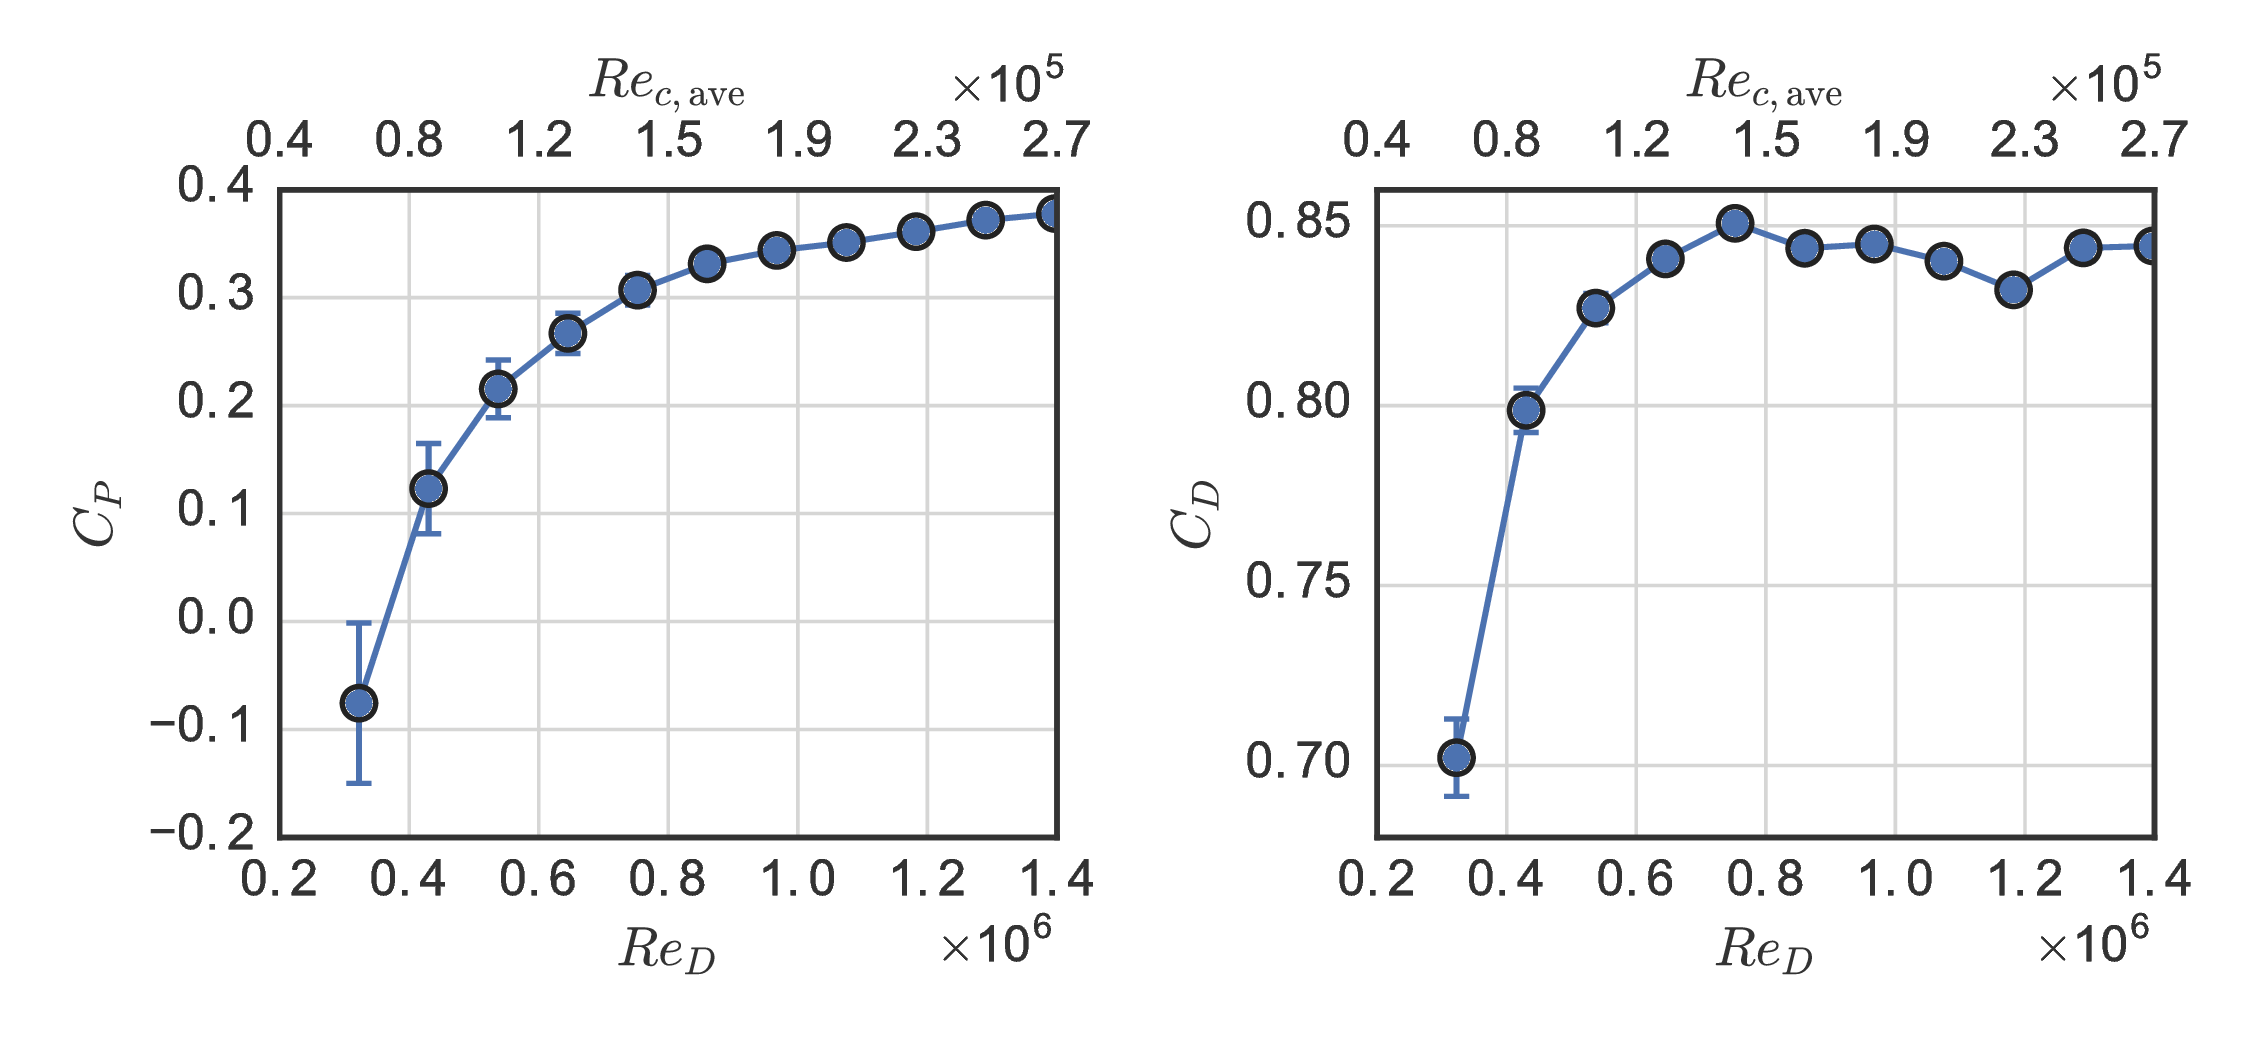
\includegraphics[width=0.85\textwidth]{RM2-tow-tank_perf_re_dep}

    \caption{Power and drag coefficient at $\lambda=3.1$ plotted versus turbine
        diameter and approximate average blade root chord Reynolds number.}

    \label{fig:perf-re-dep}
\end{figure}


\subsection{Strut drag losses}

Performance curves for the rotor with both NACA 0021 and cylindrical struts are
shown in Figure~\ref{fig:perf-covers}. As expected, the high drag cylindrical
struts reduce performance dramatically, producing an entirely negative $C_P$
curve. The detrimental effects of the strut drag were more pronounced at higher
$\lambda$. This is in accordance with the measurements of Rawlings
\cite{Rawlings2008}, though the strut losses in this case were larger due to the
very high drag circular profile. In contrast to the dramatic effect strut drag
had on $C_P$, overall rotor drag measurements were relatively similar for both
the cylindrical and NACA 0021 strut cases.

\begin{figure}
    \centering

    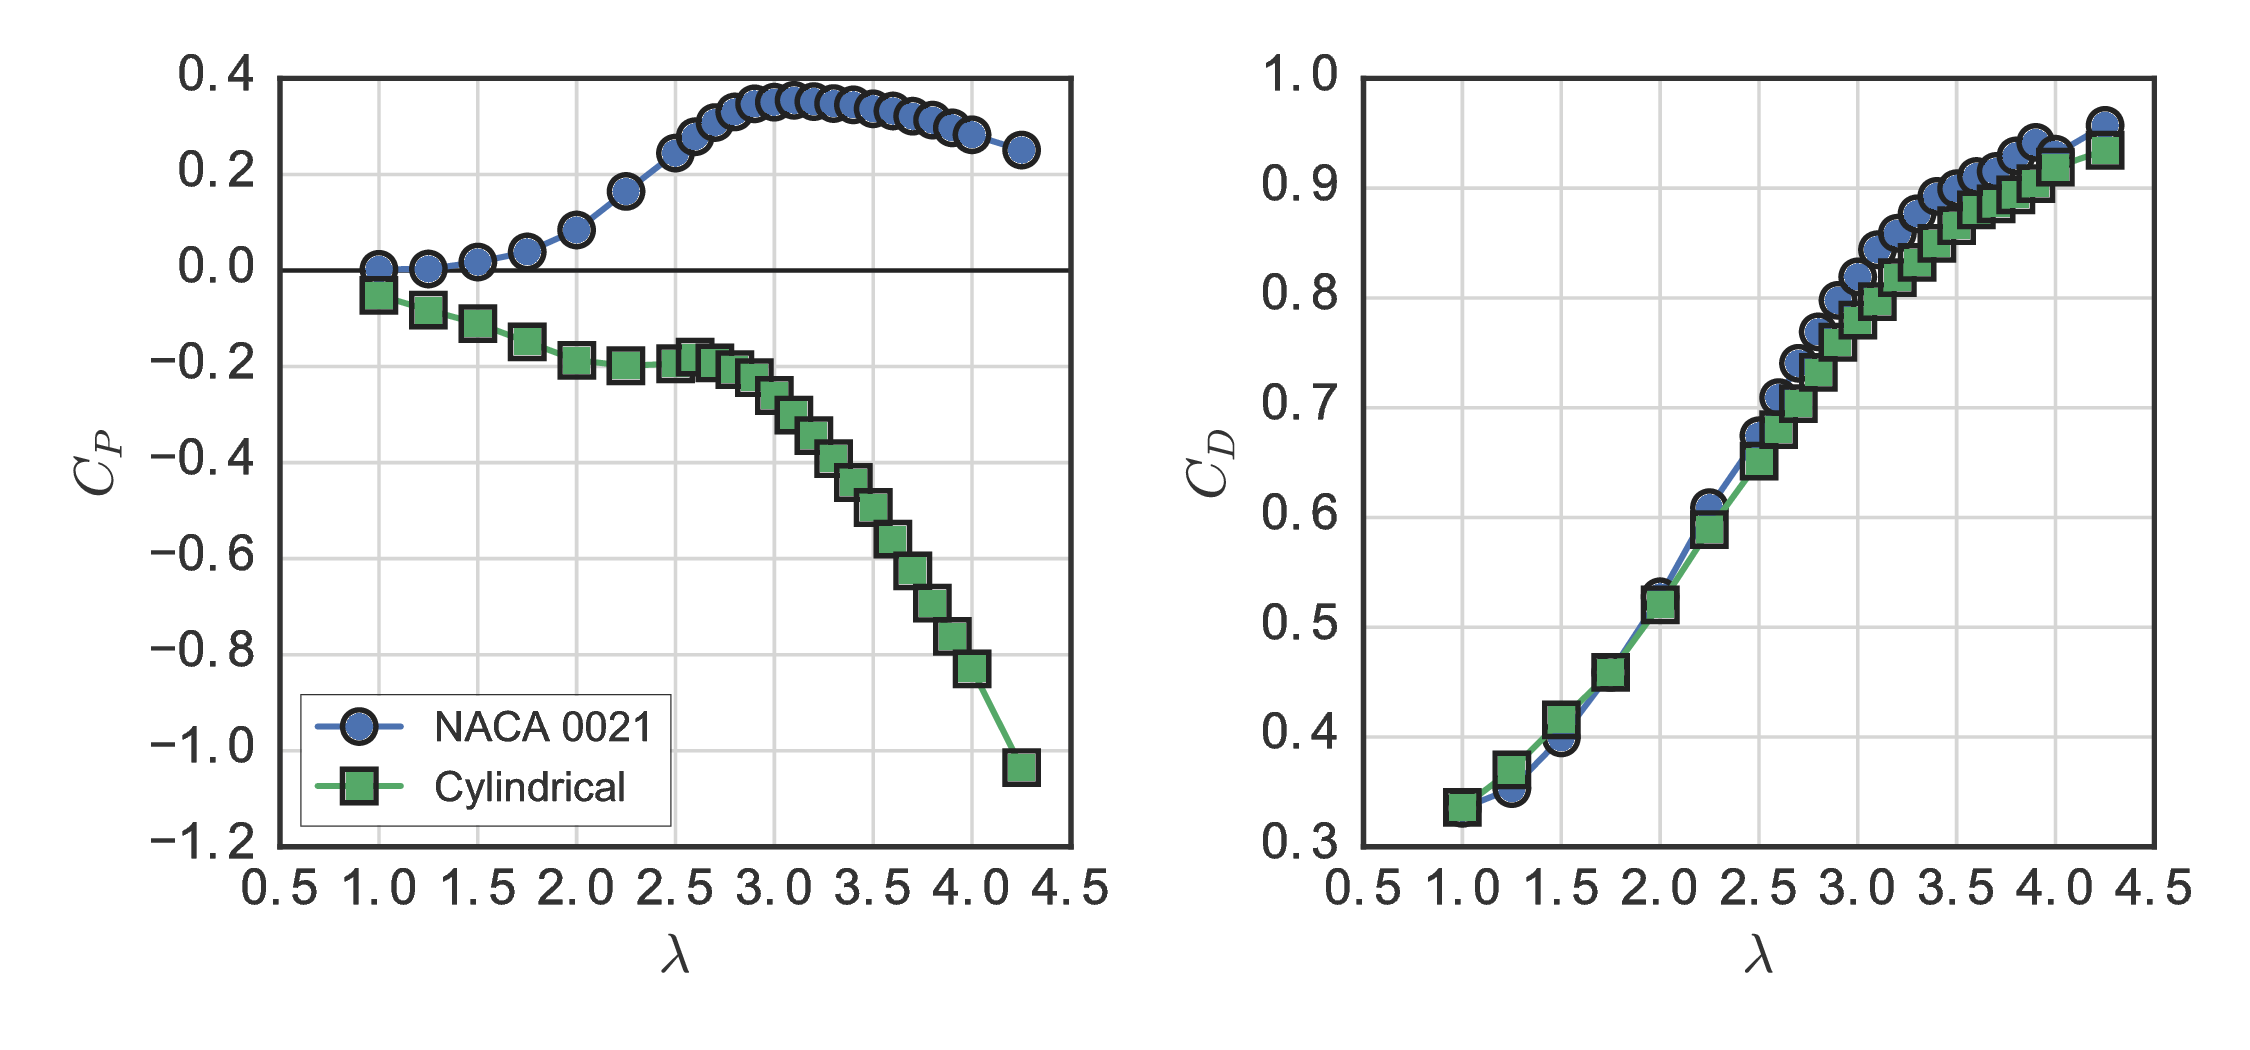
\includegraphics[width=0.9\textwidth]{RM2-tow-tank_perf_covers}

    \caption{Turbine performance and rotor drag coefficient curves with both
        NACA 0021 and cylindrical struts.}

    \label{fig:perf-covers}
\end{figure}

Measurements for the power coefficient contributions of the strut drag losses
are presented in Figure~\ref{fig:no-blades} for NACA 0021 and cylindrical
struts---both in towed and stationary conditions. These are computed in the same
fashion as the curves in Figure~\ref{fig:rm2-cp-curves}, but with the rotor
blades removed. We see that strut drag losses increase with tip speed ratio to
the power 2--3, which makes streamlined struts much more important for low
solidity turbines, given the inverse correlation between solidity and
$\lambda_0$ \cite{Templin1974}.

\begin{figure}
    \centering

    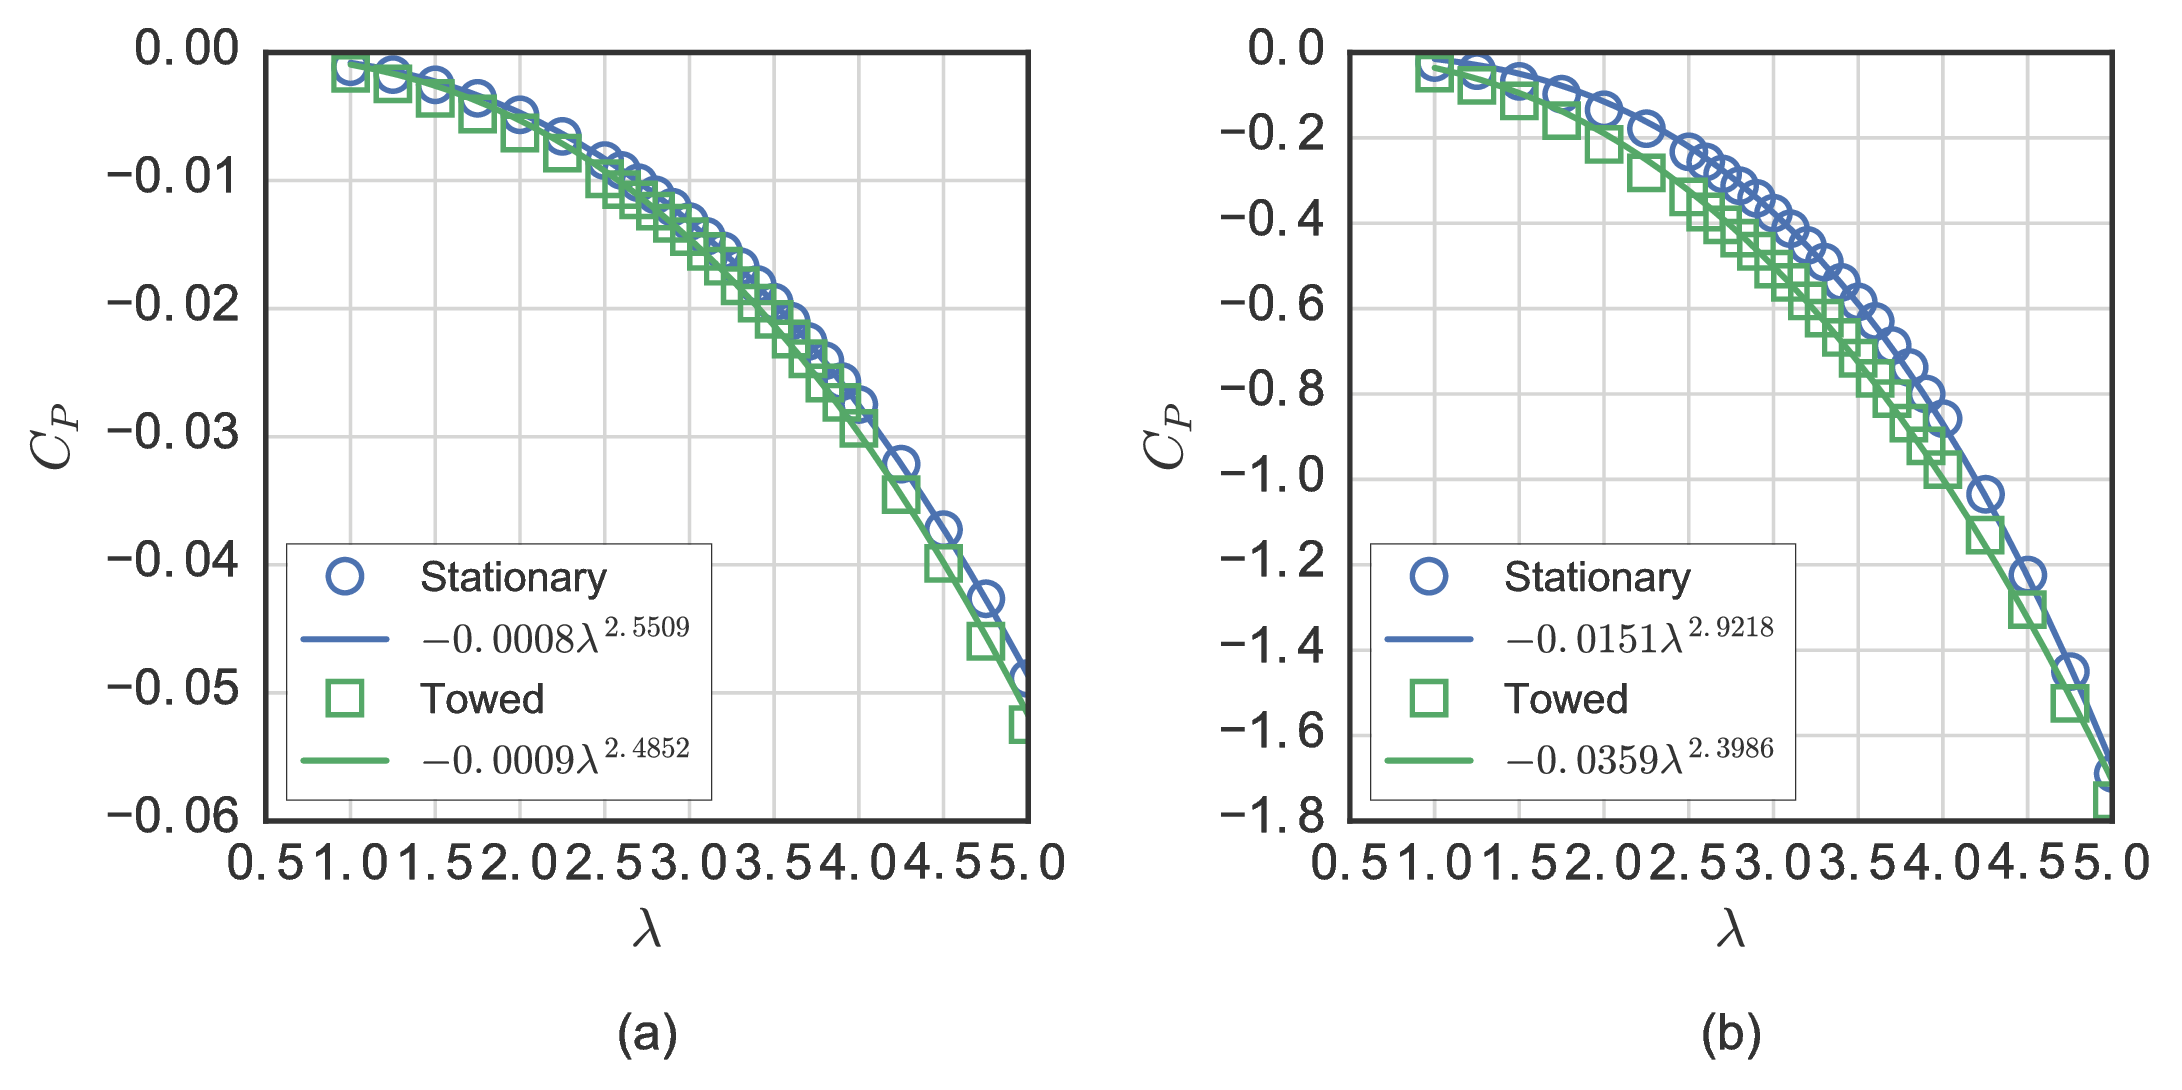
\includegraphics[width=0.9\textwidth]{RM2-tow-tank_no_blades_all}

    \caption{Measurements of the strut drag losses for (a) NACA 0021 and (b)
        cylindrical struts, both stationary and towed.}

    \label{fig:no-blades}
\end{figure}

Strut drag losses did not change much for the streamlined NACA 0021 struts in
the towed versus stationary configuration, which helps explain why overall rotor
drag coefficients remained of comparable magnitude even at low Reynolds number,
where $C_P$ was dramatically reduced, or even negative. For the cylindrical
struts, losses increased significantly when towed and operating in the mid range
of tip speed ratios.

Though a real turbine would never use such high drag struts, with respect to
numerical modeling, these measurements provide some interesting validation
cases. Modelers can isolate and evaluate the ability to predict these losses
independent of the blade loading by modeling combinations of the rotor with the
high/low drag struts and with/without blades.


\subsection{Near-wake characteristics}

The mean velocity field at the chosen optimal tip speed ratio $\lambda_0=3.1$, 1
m downstream ($x/D=0.93$) from the rotor axis is plotted in
Figure~\ref{fig:meancontquiv}. The mean streamwise velocity deficit is markedly
more symmetric than that of the higher solidity UNH-RVAT, shown in
Figure~\ref{fig:RVAT-baseline-meancontquiv}, with the RM2 inducing lower
acceleration around the turbine due to the lower rotor drag coefficient and a
slightly lower blockage ratio \cite{Bachant2015-JoT}. Tip vortex shedding is
relatively weaker, which is likely an effect of the RM2's smaller blade chord
length and tapered blades.

\begin{figure}
    \centering

    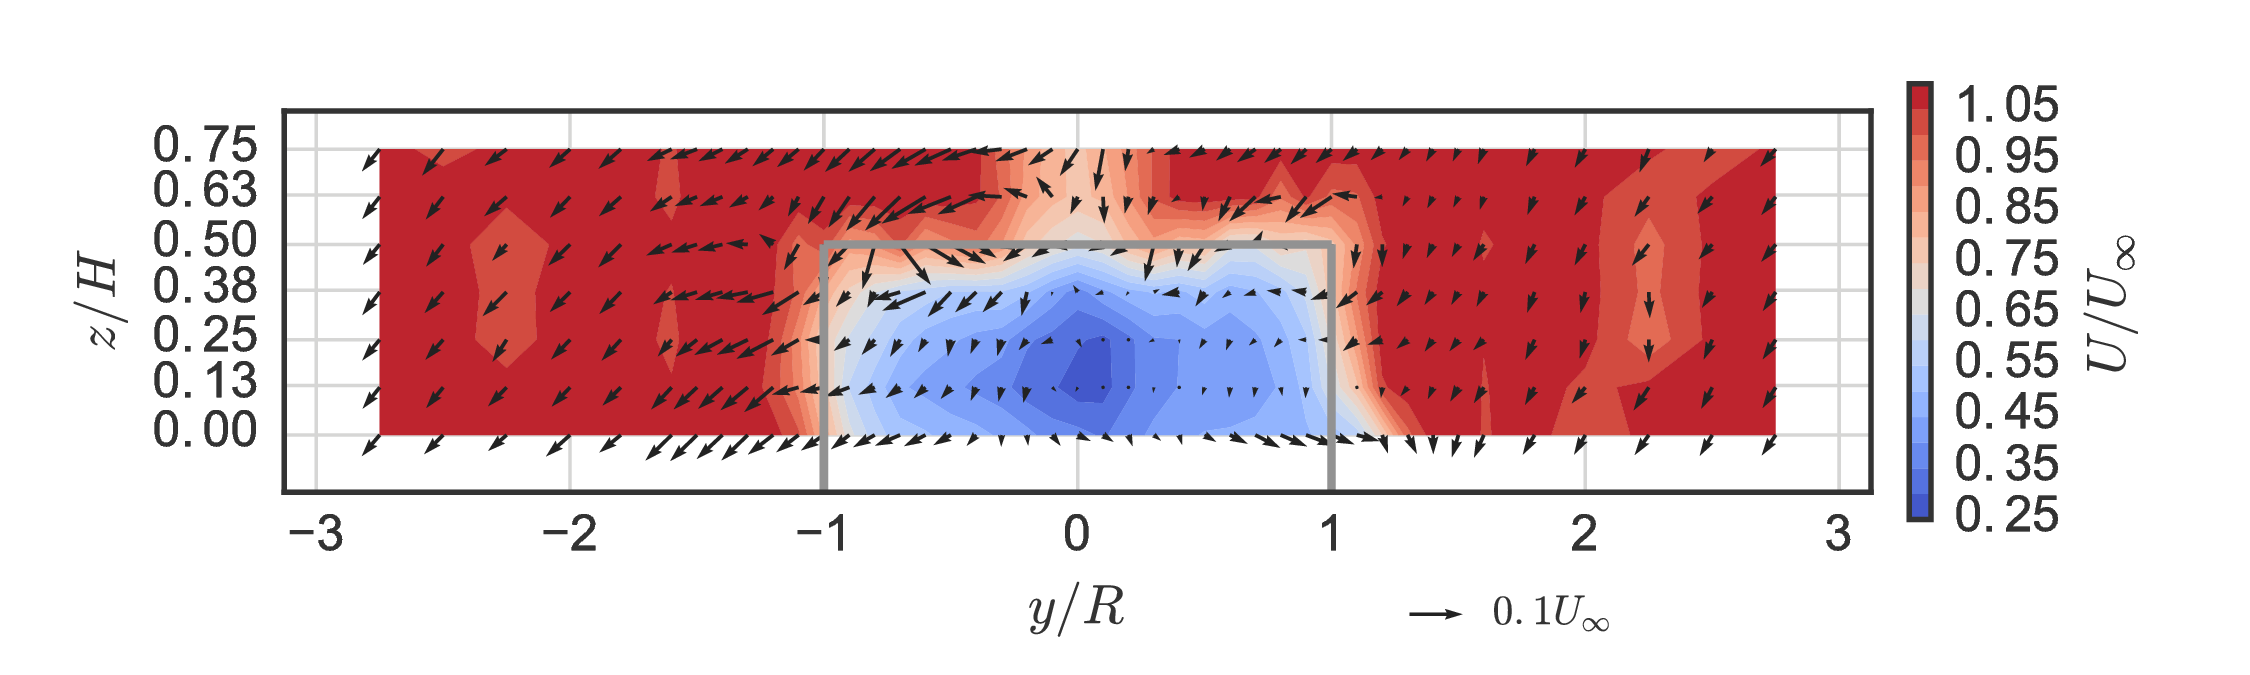
\includegraphics[width=0.9\textwidth]{RM2-tow-tank_meancontquiv}

    \caption{RM2 near-wake mean velocity field (looking upstream) at 1 m
        downstream ($x/D=0.93$), $U_\infty=1.0$ m/s, and $\lambda=3.1$. Refer to
        Figure~\ref{fig:coordinates} for turbine axis orientation. Solid dark gray
        lines indicate turbine frontal area.}

    \label{fig:meancontquiv}
\end{figure}

Figure~\ref{fig:kcont} shows the turbulence kinetic energy in the turbine wake.
We mainly see unsteadiness in the flow generated by the blade tip vortex
shedding (the horizontal band around $z/H=0.5$). Compared with the UNH-RVAT,
shown in Figure~\ref{fig:RVAT-baseline-kcont}, turbulence generation is lower
overall, without the intense vertical band around $y/R=-1$, which indicates that
the RM2 blades are operating further from stall---consistent with its higher
optimal tip speed ratio.

\begin{figure}
    \centering

    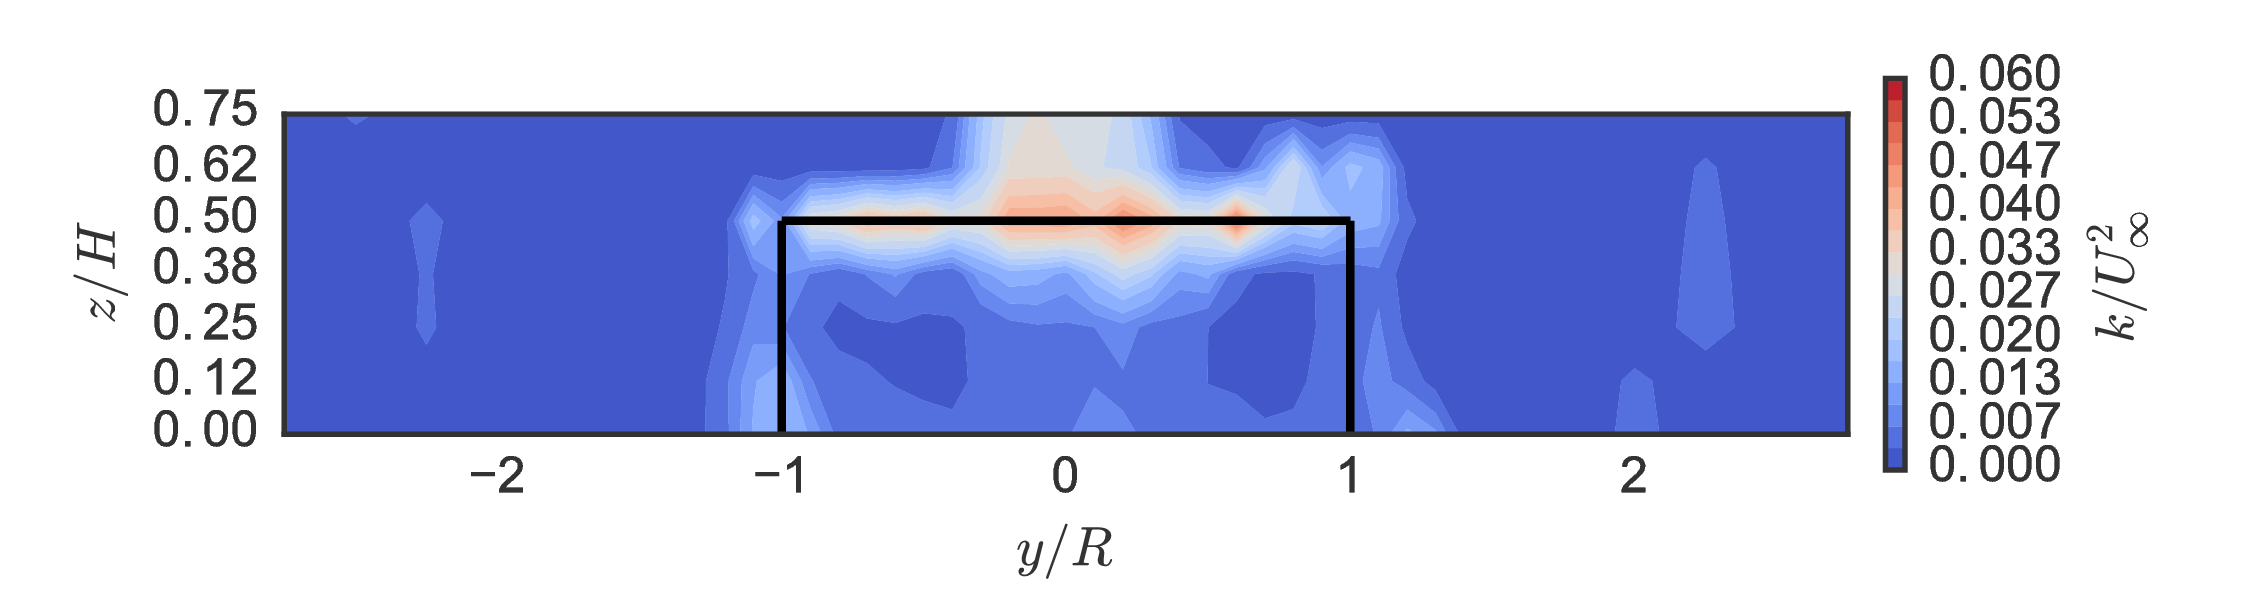
\includegraphics[width=0.9\textwidth]{RM2-tow-tank_k_contours}

    \caption{Turbulence kinetic energy in the RM2's near-wake (looking upstream)
        at 1 m downstream ($x/D=0.93$), $U_\infty=1.0$ m/s, and $\lambda=3.1$. Solid
        black lines indicate turbine frontal area.}

    \label{fig:kcont}
\end{figure}

As described in Chapter~\ref{chap:RVAT-baseline}, analysis of the near-wake of
the higher solidity UNH-RVAT turbine revealed that vertical advection was the
largest contributor to streamwise recovery \cite{Bachant2015-JoT}, a trait which
is considered an advantage of cross-flow over axial-flow rotors in arrays
\cite{Kinzel2012}. A similar analysis was undertaken for the RM2 using
Equation~\ref{eq:K-full}, the transport equation for mean kinetic energy,
rearranged to isolate the streamwise partial derivative.

Terms that were able to be calculated from the experimental data are those that
do not involve $x$-derivatives, since all wake measurement locations were at a
fixed downstream distance. The available terms are the cross-stream advection
($y$-adv.), vertical advection ($z$-adv.), transport due to turbulent
fluctuations ($y$-turb. and $z$-turb., separated by the direction of the
derivative), production of turbulence kinetic energy ($k$-prod.), and the
dissipation due to the mean velocity gradient (Mean diss.).

Derivatives were computed with a second order central difference scheme for
interior points, and a second order inward-facing scheme for the edges,
following the methodology in \cite{Bachant2015-JoT}. Weighted averages for these
calculations are shown in Figure~\ref{fig:Ktransport}. Due to the weaker blade
vortex shedding, transport due to vertical advection at this point in the wake
was approximately 3 times lower than the higher solidity UNH-RVAT. Note that
direct comparison is somewhat invalid, since the total measurement plane area
was about 5\% lower for this experiment. However, the differences observed are
larger than the area ratio between the two experiments. We also see relatively
lower levels of cross-stream turbulent transport due to the lack of blade stall
vortex shedding. These results may have interesting implications regarding the
application of turbines with lower power coefficient to possibly improve overall
array performance through enhanced transport of kinetic energy from the free
stream, though evaluating these trade-offs will require a detailed analysis of
the downstream evolution and turbine--wake interaction.

\begin{figure}
    \centering

    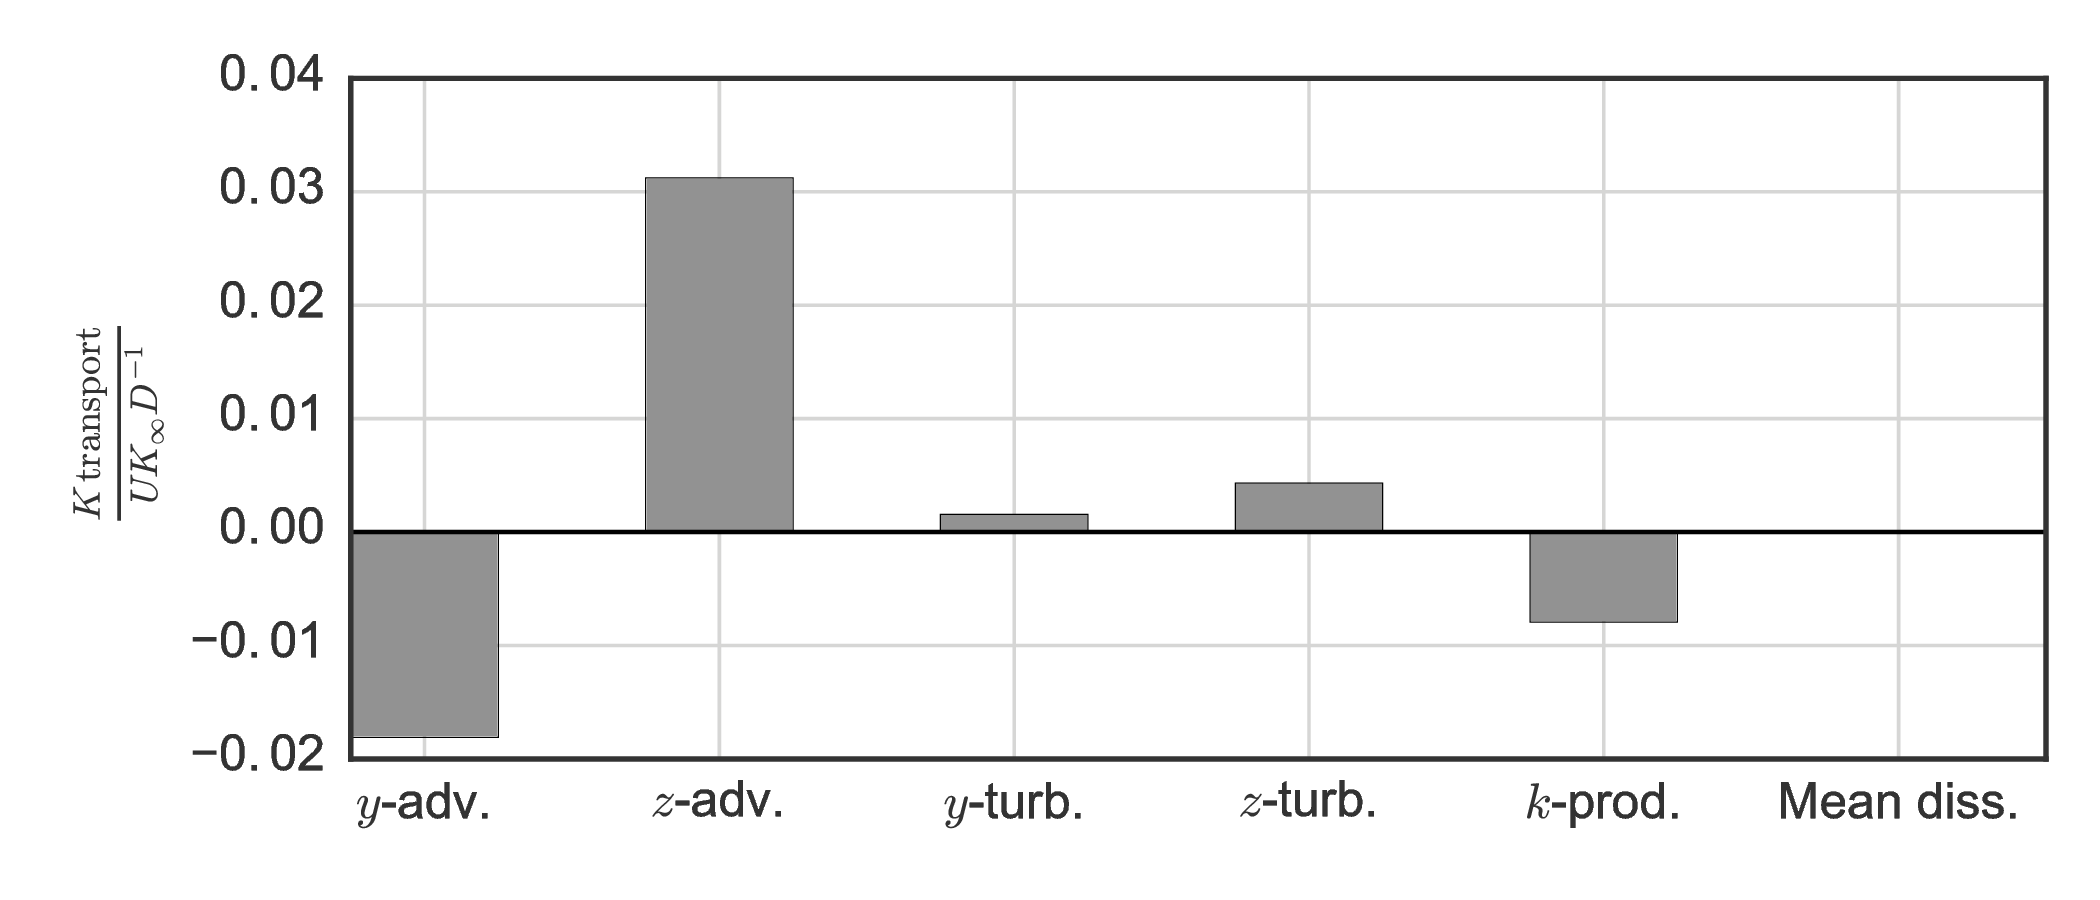
\includegraphics[width=0.9\textwidth]{RM2-tow-tank_K_trans_bar_graph}

    \caption{Weighted average estimates for terms contributing to streamwise
        recovery of mean kinetic energy, multiplied by two due to implied symmetry.}

    \label{fig:Ktransport}
\end{figure}


\section{Conclusions}

The performance and near-wake velocity of a 1:6 scale DOE Reference Model 2
cross-flow turbine were measured in a towing tank. A maximum power coefficient
$C_P = 0.37$ and rotor drag coefficient $C_D = 0.84$ were observed at an optimal
tip speed ratio $\lambda_0 = 3.1$.

Performance was assessed for Reynolds number dependence, showing a convergence
to a weakly $Re$-dependent linear regime at approximately $Re_D \approx 1 \times
10^6$ or $Re_{c,\mathrm{ave}} \approx 2 \times 10^5$. Comparison was made
between this turbine and the higher solidity UNH-RVAT, tested in nearly
identical conditions, which showed similar Reynolds number thresholds but a
flatter linear regime, likely to due virtual camber of the higher
chord-to-radius ratio of the UNH-RVAT blades. Nevertheless, these results
indicate an important transitional scale threshold beyond which data should be
taken for numerical model validation, in order to stay relevant to full scale
devices.

The effects of parasitic drag from blade support struts on turbine performance
were measured by rotating the turbine without blades while stationary and while
towing. These losses---even for a streamlined hydrofoil strut---can become
significant at higher tip speed ratios---up to an approximate 5 percentage point
decrease in power coefficient at a tip speed ratio of 5. These measurements were
repeated with a set of high-drag cylindrical struts, which as expected,
prevented the turbine from producing any mechanical power at any tip speed
ratio. Nevertheless these measurements provide useful validation data for both
high and low fidelity numerical performance prediction models, allowing
researchers and engineers to test predictions without blade effects.

While operating at its optimal tip speed ratio $\lambda=3.1$ the wake at
$x/D=0.93$ downstream was shown to be relatively symmetrical and lacked the
evidence of strong blade stall, both of which differentiate this near-wake from
the higher solidity, lower $\lambda_0$ UNH-RVAT. Terms from the mean kinetic
energy transport equation were also computed in this $y$--$z$ plane, showing the
relative importance of the vertical advection compared with turbulent transport
terms at this location, which is qualitatively similar to the UNH-RVAT wake
data. However, lower wake recovery totals were calculated. This indicates that
although the RM2 is a more effective energy converter than the UNH-RVAT, its
wake recovery may in fact be delayed due to weaker blade tip vortex shedding and
lower levels of turbulence in the near-wake, which may present a trade-off when
considering optimal array layouts.

This dataset, along with the code for processing and visualization, is provided
openly via a Creative Commons license (MIT license for code), and is available
as a Git repository from \url{http://github.com/UNH-CORE/RM2-tow-tank} or a
citable archive \cite{Bachant2016-RM2-data}. Note that the processing code will
automatically download raw data as necessary so users can perform a full
reanalysis of the measurements presented here.


\section{Acknowledgments}

This study was carried out in collaboration with Sandia National Laboratories
and was supported by the Department of Energy (DOE), Office of Energy Efficiency
and Renewable Energy (EERE), Wind and Water Power Technologies Office (WWPTO).
Sandia National Laboratories is a multi-program laboratory managed and operated
by Sandia Corporation, a wholly owned subsidiary of Lockheed Martin Corporation,
for the U.S. Department of Energy's National Nuclear Security Administration
under contract DE-AC04-94AL85000.
